\chapter{Analiza tematu}

\section{Struktury systemów}

Typy systemów ANC dzielimy głównie ze względu 
rodzaj wykorzystywanego sterowania, z którego wyróżniamy:

\begin{enumerate}

    \item Sterowanie ze sprzężeniem w przód - hałas jest mierzony przed
    dotarciem do aktuatora (głośnika), a następnie mierzony ponownie
    za aktuatorem w celu określenia, jak bardzo został wytłumiony.

    \item Sterowanie ze sprzężeniem w tył - hałas jest mierzony jedynie
    za aktuatorem.

\end{enumerate}

Hałas występujący przed aktuatorem nazywamy hałasem pierwotnym i w 
nomenklaturze automatyki traktowany jako wejście systemu, gdzie 
ten mierzony za aktuatorem, nazywany hałasem resztkowym, traktowany jest jak błąd (uchyb).
W związku z przyjęciem takiego nazewnictwa, można napisać,
że systemy ANC ze sprzężeniem w przód opierają swoje działanie na pomiarze
wejścia i błędu, a system ze sprzężeniem w tył tylko na pomiarze błędu.

\begin{figure}[H]
    \centering
    \begin{subfigure}[b]{0.49\textwidth}
        \centering
        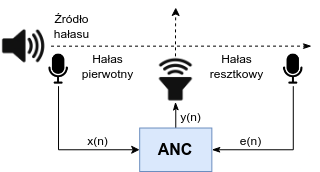
\includegraphics[width=\textwidth]{graf/analysis/bb_fw_anc.png}
        \caption{ANC ze sprzężeniem w przód}
    \end{subfigure}
    \hfill
    \begin{subfigure}[b]{0.49\textwidth}
        \centering
        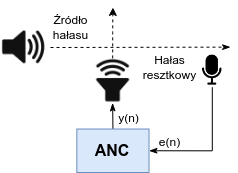
\includegraphics[width=0.75\textwidth]{graf/analysis/fb_anc.png}
        \caption{ANC ze sprzężeniem w tył}
    \end{subfigure}
       \caption{Porównanie struktur systemów}
       \label{analysis::structs}
\end{figure}

\par Instynktownie można stwierdzić, że skoro systemy ze sprzężeniem w przód
opierają swoje działanie na pomiarze dwóch wielkości, to ze względu 
na większą ilość informacji, sterowanie może zostać wypracowane z większą
dokładnością. Jest to stwierdzenie poprawne, jednak należy pamiętać,
że takie układy wymagają dodatkowego pomiaru (czujnika),
co zwiększa koszta oraz komplikuje strukturę.
Dodatkowy pomiar jest też nie zawsze możliwy, więc wybór struktury często
jest kompromisem.

\par Projektujac układ ze sprzężeniem w przód można dokonać dodatkowych
założeń, które implikują dwa podtypy struktur. Założenia opierają
się na charakterystyce hałasu pierwotnego, na podstawie której można zdefiniować: 

\begin{enumerate}

    \item Hałas szerokopasmowy - losowy, wywołany przez niespodziewane
    zaburzenia ośrodka. Jako, że jest losowy, jego energia jest 
    równomiernie rozprowadzona w całym paśmie częstotliwości.

    \item Hałas wąskopasmowy - skoncentrowany w specifycznych pasmach.
    Może być wywołany przez maszyny pracujące w sposób okresowy,
    przykładowo silniki lub obracające się wały. W związku, że praca
    takich elementów jest periodyczna, to hałas, który dystrybuują, również.

\end{enumerate}

W każdym przypadku wymagane jest, że element pomiarowy mierzący
hałas na wejściu systemu będzie zdolny zapewnić odpowiednią ilość informacji
do wytworzenia adekwatnego sterowania. W przypadku hałasów szerokopasmowych
wybór pada na mikrofon referencyjny, w przypadku hałasów wąskopasmowych 
z mikrofonu można zrezygonować na rzecz czujnika nieakustycznego,
takiego jak tachometr lub enkoder, kiedy mamy do czynienia z hałasami wygenerowanymi 
przez obracający się mechanizm.




\section{Proponowane rozwiązanie}
